

\tikzset{every picture/.style={line width=0.75pt}} %set default line width to 0.75pt        

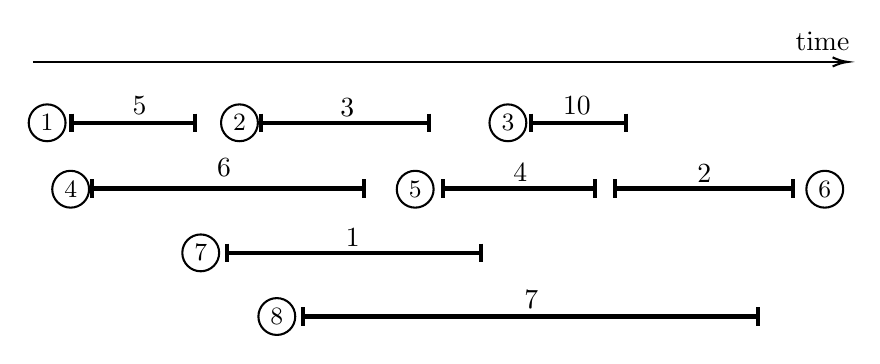
\begin{tikzpicture}[x=0.5pt,y=0.5pt,yscale=-1,xscale=1]
%uncomment if require: \path (0,248); %set diagram left start at 0, and has height of 248

%Straight Lines [id:da9015649955021968] 
\draw    (7,37) -- (594,37) ;
\draw [shift={(596,37)}, rotate = 180] [color={rgb, 255:red, 0; green, 0; blue, 0 }  ][line width=0.75]    (10.93,-3.29) .. controls (6.95,-1.4) and (3.31,-0.3) .. (0,0) .. controls (3.31,0.3) and (6.95,1.4) .. (10.93,3.29)   ;
%Straight Lines [id:da9640237890291299] 
\draw [line width=1.5]    (35,81) -- (124.5,81) ;
\draw [shift={(124.5,81)}, rotate = 180] [color={rgb, 255:red, 0; green, 0; blue, 0 }  ][line width=1.5]    (0,6.71) -- (0,-6.71)   ;
\draw [shift={(35,81)}, rotate = 180] [color={rgb, 255:red, 0; green, 0; blue, 0 }  ][line width=1.5]    (0,6.71) -- (0,-6.71)   ;
%Straight Lines [id:da3355888679808179] 
\draw [line width=1.5]    (172,81) -- (293.5,81) ;
\draw [shift={(293.5,81)}, rotate = 180] [color={rgb, 255:red, 0; green, 0; blue, 0 }  ][line width=1.5]    (0,6.71) -- (0,-6.71)   ;
\draw [shift={(172,81)}, rotate = 180] [color={rgb, 255:red, 0; green, 0; blue, 0 }  ][line width=1.5]    (0,6.71) -- (0,-6.71)   ;
%Straight Lines [id:da09988799250468405] 
\draw [line width=1.5]    (367,81) -- (435.5,81) ;
\draw [shift={(435.5,81)}, rotate = 180] [color={rgb, 255:red, 0; green, 0; blue, 0 }  ][line width=1.5]    (0,6.71) -- (0,-6.71)   ;
\draw [shift={(367,81)}, rotate = 180] [color={rgb, 255:red, 0; green, 0; blue, 0 }  ][line width=1.5]    (0,6.71) -- (0,-6.71)   ;
%Straight Lines [id:da4026459071674142] 
\draw [line width=1.5]    (50,128.5) -- (246.5,128.5) ;
\draw [shift={(246.5,128.5)}, rotate = 180] [color={rgb, 255:red, 0; green, 0; blue, 0 }  ][line width=1.5]    (0,6.71) -- (0,-6.71)   ;
\draw [shift={(50,128.5)}, rotate = 180] [color={rgb, 255:red, 0; green, 0; blue, 0 }  ][line width=1.5]    (0,6.71) -- (0,-6.71)   ;
%Straight Lines [id:da5509115882034084] 
\draw [line width=1.5]    (303.5,128.5) -- (413.5,128.5) ;
\draw [shift={(413.5,128.5)}, rotate = 180] [color={rgb, 255:red, 0; green, 0; blue, 0 }  ][line width=1.5]    (0,6.71) -- (0,-6.71)   ;
\draw [shift={(303.5,128.5)}, rotate = 180] [color={rgb, 255:red, 0; green, 0; blue, 0 }  ][line width=1.5]    (0,6.71) -- (0,-6.71)   ;
%Straight Lines [id:da6271509388583772] 
\draw [line width=1.5]    (428,128.5) -- (556.5,128.5) ;
\draw [shift={(556.5,128.5)}, rotate = 180] [color={rgb, 255:red, 0; green, 0; blue, 0 }  ][line width=1.5]    (0,6.71) -- (0,-6.71)   ;
\draw [shift={(428,128.5)}, rotate = 180] [color={rgb, 255:red, 0; green, 0; blue, 0 }  ][line width=1.5]    (0,6.71) -- (0,-6.71)   ;
%Straight Lines [id:da26802882985941956] 
\draw [line width=1.5]    (147.5,175) -- (331,175) ;
\draw [shift={(331,175)}, rotate = 180] [color={rgb, 255:red, 0; green, 0; blue, 0 }  ][line width=1.5]    (0,6.71) -- (0,-6.71)   ;
\draw [shift={(147.5,175)}, rotate = 180] [color={rgb, 255:red, 0; green, 0; blue, 0 }  ][line width=1.5]    (0,6.71) -- (0,-6.71)   ;
%Straight Lines [id:da22029647624095072] 
\draw [line width=1.5]    (202.5,221) -- (531,221) ;
\draw [shift={(531,221)}, rotate = 180] [color={rgb, 255:red, 0; green, 0; blue, 0 }  ][line width=1.5]    (0,6.71) -- (0,-6.71)   ;
\draw [shift={(202.5,221)}, rotate = 180] [color={rgb, 255:red, 0; green, 0; blue, 0 }  ][line width=1.5]    (0,6.71) -- (0,-6.71)   ;

% Text Node
\draw (556,13) node [anchor=north west][inner sep=0.75pt]   [align=left] {time};
% Text Node
\draw    (17.38, 81) circle [x radius= 13.31, y radius= 13.31]   ;
\draw (17.38,81) node  [font=\small] [align=left] {$\displaystyle 1$};
% Text Node
\draw    (156.38, 81) circle [x radius= 13.31, y radius= 13.31]   ;
\draw (156.38,81) node  [font=\small] [align=left] {$\displaystyle 2$};
% Text Node
\draw    (350.38, 81) circle [x radius= 13.31, y radius= 13.31]   ;
\draw (350.38,81) node  [font=\small] [align=left] {$\displaystyle 3$};
% Text Node
\draw    (34.38, 129) circle [x radius= 13.31, y radius= 13.31]   ;
\draw (34.38,129) node  [font=\small] [align=left] {$\displaystyle 4$};
% Text Node
\draw    (283.38, 129) circle [x radius= 13.31, y radius= 13.31]   ;
\draw (283.38,129) node  [font=\small] [align=left] {$\displaystyle 5$};
% Text Node
\draw    (579.38, 129) circle [x radius= 13.31, y radius= 13.31]   ;
\draw (579.38,129) node  [font=\small] [align=left] {$\displaystyle 6$};
% Text Node
\draw    (128.38, 175) circle [x radius= 13.31, y radius= 13.31]   ;
\draw (128.38,175) node  [font=\small] [align=left] {$\displaystyle 7$};
% Text Node
\draw    (183.38, 221) circle [x radius= 13.31, y radius= 13.31]   ;
\draw (183.38,221) node  [font=\small] [align=left] {$\displaystyle 8$};
% Text Node
\draw (77,60) node [anchor=north west][inner sep=0.75pt]   [align=left] {$\displaystyle 5$};
% Text Node
\draw (227,61) node [anchor=north west][inner sep=0.75pt]   [align=left] {$\displaystyle 3$};
% Text Node
\draw (388,60) node [anchor=north west][inner sep=0.75pt]   [align=left] {$\displaystyle 10$};
% Text Node
\draw (138,105) node [anchor=north west][inner sep=0.75pt]   [align=left] {$\displaystyle 6$};
% Text Node
\draw (352,108) node [anchor=north west][inner sep=0.75pt]   [align=left] {$\displaystyle 4$};
% Text Node
\draw (485,109) node [anchor=north west][inner sep=0.75pt]   [align=left] {$\displaystyle 2$};
% Text Node
\draw (231,155) node [anchor=north west][inner sep=0.75pt]   [align=left] {$\displaystyle 1$};
% Text Node
\draw (360,200) node [anchor=north west][inner sep=0.75pt]   [align=left] {$\displaystyle 7$};


\end{tikzpicture}

